\documentclass[12pt,letterpaper]{exam}
\usepackage[lmargin=1in,rmargin=1in,tmargin=1in,bmargin=1in]{geometry}
\usepackage{../style/exams}

% -------------------
% Course & Exam Information
% -------------------
\newcommand{\course}{MAT 101: Exam 1}
\newcommand{\term}{Spring --- 2024}
\newcommand{\examdate}{02/21/2024}
\newcommand{\timelimit}{85 Minutes}

\setbool{hideans}{false} % Student: True; Instructor: False

% -------------------
% Content
% -------------------
\begin{document}

\examtitle
\instructions{Write your name on the appropriate line on the exam cover sheet. This exam contains \numpages\ pages (including this cover page) and \numquestions\ questions. Check that you have every page of the exam. Answer the questions in the spaces provided on the question sheets. Be sure to answer every part of each question and show all your work. If you run out of room for an answer, continue on the back of the page --- being sure to indicate the problem number.} 
\scores
\bottomline
\newpage


% -------------------
% Questions
% -------------------
\begin{questions}

% Question 1
\newpage
\question[10] Consider the relation given by the diagram below.
	\[
	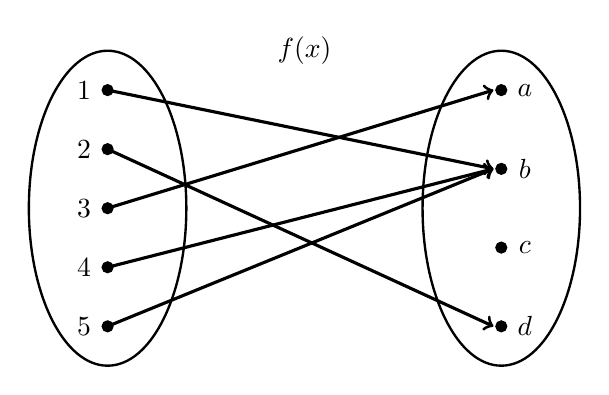
\begin{tikzpicture}
	\node at (2.5,2) {$f(x)$};
	
	% Ellipses
	\draw[line width=0.03cm] (0,0) circle (1 and 2);
	\draw[line width=0.03cm] (5,0) circle (1 and 2);
	
	% Nodes
	\draw[fill=black] (0,1.5) circle (0.07);
	\draw[fill=black] (0,0.75) circle (0.07);
	\draw[fill=black] (0,0) circle (0.07);
	\draw[fill=black] (0,-0.75) circle (0.07);
	\draw[fill=black] (0,-1.5) circle (0.07);
	
	\draw[fill=black] (5,1.5) circle (0.07);
	\draw[fill=black] (5,0.50) circle (0.07);
	\draw[fill=black] (5,-0.5) circle (0.07);
	\draw[fill=black] (5,-1.5) circle (0.07);
	
	% Arrow
	\draw[line width=0.04cm,->] (0,1.5) -- (4.9,0.50);
	\draw[line width=0.04cm,->] (0,0.75) -- (4.9,-1.5);
	\draw[line width=0.04cm,->] (0,0) -- (4.9,1.5);
	\draw[line width=0.04cm,->] (0,-1.5) -- (4.9,0.5);
	\draw[line width= 0.04cm,->,black] (0,-0.75) -- (4.9,0.5);
	
	% Labels
	\node at (-0.3,1.5) {$1$};
	\node at (-0.3,0.75) {$2$};
	\node at (-0.3,0) {$3$};
	\node at (-0.3,-0.75) {$4$};
	\node at (-0.3,-1.5) {$5$};
	
	\node at (5.3,1.5) {$a$};
	\node at (5.3,0.5) {$b$};
	\node at (5.3,-0.5) {$c$};
	\node at (5.3,-1.5) {$d$};
	\end{tikzpicture}
	\]

\begin{enumerate}[(a)]
\item Is the relation a function? Explain. 
\item Find the domain of the relation.
\item Find the codomain of the relation.
\item Find the range of the relation. 
\end{enumerate} \pspace

\sol
\begin{enumerate}[(a)]
\item Yes, the relation $f(x)$ is a function. Observe for that each of its inputs, $1, 2, 3, 4, 5$, there is exactly one output, $a, b, c, d$, respectively. \pspace

\item The domain of this function is $\{ 1, 2, 3, 4, 5 \}$. \pspace

\item The codomain of this function is $\{ a, b, c, d \}$. \pspace

\item The range or image of this function is $\{ a, b, d \}$. 
\end{enumerate}



% Question 2
\newpage
\question[10] Consider the relation plotted below.
	\[
	\fbox{
	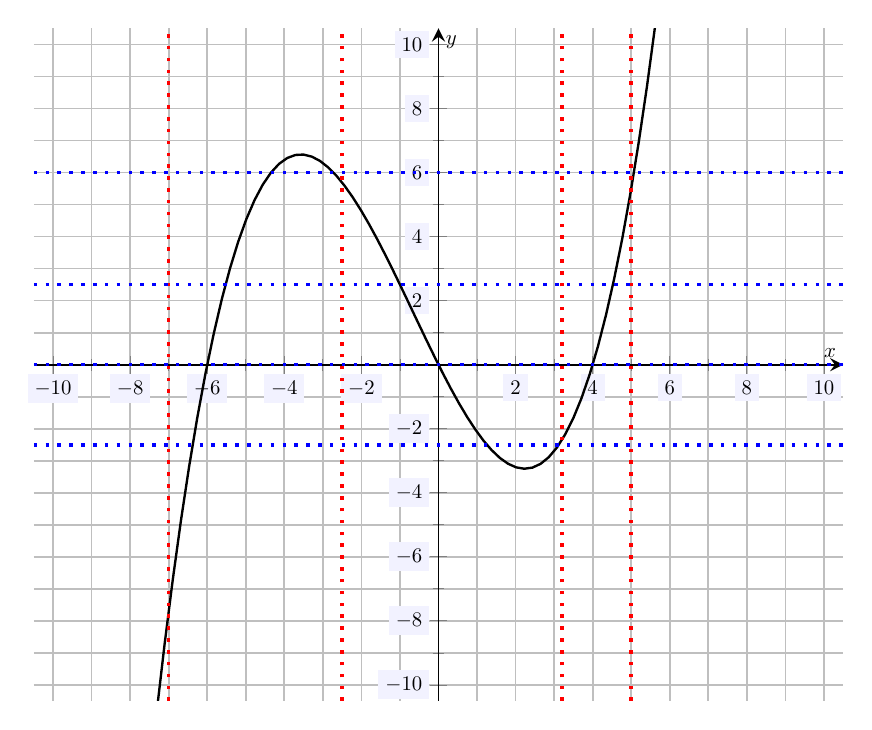
\begin{tikzpicture}[scale=1.5,every node/.style={scale=0.5}]
	\begin{axis}[
	grid=both,
	axis lines=middle,
	ticklabel style={fill=blue!5!white},
	xmin= -10.5, xmax=10.5,
	ymin= -10.5, ymax=10.5,
	xtick={-10,-8,-6,-4,-2,0,2,4,6,8,10},
	ytick={-10,-8,-6,-4,-2,0,2,4,6,8,10},
	minor tick = {-10,-9,...,10},
	xlabel=\(x\),ylabel=\(y\),
	]
	\addplot[line width= 0.02cm,samples=100,domain= -10.5:10.5] ({x},{1/10*x*(x + 6)*(x-4)});
	
	\draw[line width=0.03cm,dotted,red] (-7,-10.5) -- (-7,10.5);
	\draw[line width=0.03cm,dotted,red] (-2.5,-10.5) -- (-2.5,10.5);
	\draw[line width=0.03cm,dotted,red] (3.2,-10.5) -- (3.2,10.5);
	\draw[line width=0.03cm,dotted,red] (5,-10.5) -- (5,10.5);
	
	\draw[line width=0.03cm,dotted,blue] (-10.5,6) -- (10.5,6);
	\draw[line width=0.03cm,dotted,blue] (-10.5,2.5) -- (10.5,2.5);
	\draw[line width=0.03cm,dotted,blue] (-10.5,0) -- (10.5,0);
	\draw[line width=0.03cm,dotted,blue] (-10.5,-2.5) -- (10.5,-2.5);
	\end{axis}
	\end{tikzpicture}
	}
	\] 

\begin{enumerate}[(a)]
\item Is this relation a function of $x$? Explain.
\item Is this relation a function of $y$? Explain. 
\item If one were to consider this relation as a function of $x$, would the relation have an inverse? Explain. 
\end{enumerate} \pspace

\sol 
\begin{enumerate}[(a)]
\item Yes, this relation is a function of $x$. This is because the relation passes the vertical line test; that is, every vertical line intersects the graph of the relation at most once. Therefore, for each $x$, there is at most once $y$-value associated to $x$. \pspace

\item No, the relation is not a function of $y$. This is because the relation fails the horizontal line test; that is, there is a horizontal line that intersects the graph of the relation more than once. Therefore, there is a $y$-value that is associated to more than one $x$-value. For instance, the $y$-value $0$ is associated to $x= -6, 0, 4$. \pspace

\item No, the relation would not have an inverse. This is because the relation fails the horizontal line test; that is, there is a horizontal line that intersects the graph of the relation more than once. Therefore, there is a $y$-value that is associated to more than one $x$-value. For instance, the $y$-value $0$ is associated to $x= -6, 0, 4$, i.e. if we called this relation $f(x)$ then $f^{-1}(0)= \{ -6, 0, 4 \}$. 
\end{enumerate}



% Question 3
\newpage
\question[10] Let $f(x)$ be the relation given by $f(x)= x(x - 1)(x + 3)$. 
	\begin{enumerate}[(a)]
	\item Is $f(x)$ a function? Explain. 
	\item Find $f(2)$.
	\item Find the $y$-intercept(s) of $f(x)$. 
	\item Find the $x$-intercept(s) of $f(x)$.
	\end{enumerate} \pspace

\sol 
\begin{enumerate}[(a)]
\item Yes, the relation is a function. For each input $x$, there is exactly one output---namely, the one obtained by evaluating $f(x)$ at $x$ and following order of operations. \pspace

\item We have\dots
	\[
	f(2)= 2(2 - 1)(2 + 3)= 2(1)5= 10
	\] \pspace

\item The $y$-intercept is the point where the graph of $f(x)$ intersects the $y$-axis, where $x= 0$. But then\dots
	\[
	f(0)= 0(0 - 1)(0 + 3)= 0(-1)3= 0
	\]
Therefore, the $y$-intercept is $0$, i.e. the point $(0, 0)$. \pspace

\item The $x$-intercepts are the point(s) where the graph of $f(x)$ intersects the $x$-axis, where $y= 0$. But then\dots
	\[
	\begin{aligned}
	f(x)= 0 \\
	x(x - 1)(x + 3)= 0
	\end{aligned}
	\]
This implies that either $x= 0$, or $x - 1=0$ so that $x= 1$, or $x + 3= 0$ so that $x= -3$. Therefore, the $x$-intercepts are $-3, 0, 1$, i.e. the points $(-3, 0)$, $(0, 0)$, and $(1, 0)$. 
\end{enumerate}



% Question 4
\newpage
\question[10] Let $f(x)$ and $g(x)$ be functions for which a table of values is given below. \par
	\begin{table}[ht]
	\centering
	\begin{tabular}{|c||c|c|c|c|c|c|} \hline 
	$x$ & $-5$ & $-2$ & $0$ & $1$ & $2$ & $3$ \\ \hline \hline
	$f(x)$ & $\phantom{-}6$ & $-1$ & $\phantom{-}3$ & $4$ & $3$ & $-1$ \\ \hline
	$g(x)$ & $-5$ & $\phantom{-}7$ & $-2$ & $4$ & $0$ & $\phantom{-}6$ \\ \hline 
	\end{tabular}
	\end{table} \par
Based on the table above, compute the following:
	\begin{enumerate}[(a)]
	\item $f(-2) - g(3)$
	\item $(f + g)(2)$
	\item $(fg)(-5)$
	\item $(g \circ f)(0)$
	\item $(f \circ g)(0)$
	\end{enumerate} \pspace

\sol 
\begin{enumerate}[(a)]
\item 
	\[
	f(-2) - g(3)= -1 - 6= -7
	\] \pspace 

\item 
	\[
	(f + g)(2)= f(2) + g(2)= 3 + 0= 3
	\] \pspace 

\item 
	\[
	(fg)(-5)= f(-5) \cdot g(-5)= 6 \cdot -5= -30
	\] \pspace 

\item 
	\[
	(g \circ f)(0)= g \big( f(0) \big)= g(3)= 6
	\] \pspace 

\item 
	\[
	(f \circ g)(0)= f \big( g(0) \big)= f(-2)= -1
	\]  
\end{enumerate}



% Question 5
\newpage
\question[10] Let $g(x)= x^2 + 2x - 3$. 
	\begin{enumerate}[(a)]
	\item Find $g(2)$ and $g(-4)$.
	\item Based on your answer to (a), can $g^{-1}(x)$ exist? Explain. 
	\end{enumerate} \pspace

\sol 
\begin{enumerate}[(a)]
\item We have\dots
	\[
	\begin{aligned}
	g(2)&= 2^2 + 2(2) - 3= 4 + 4 - 3= 5 \\
	g(-4)&= (-4)^2 + 2(-4) - 3= 16 - 8 - 3= 5
	\end{aligned}
	\] \pspace

\item No, $g^{-1}(x)$ cannot exist. We know that $g(2)= 5= g(-4)$. Therefore, $g^{-1}(5)$ contains the set $\{ -4, 2 \}$, i.e. the input $5$ would have more than one output. Therefore, $g^{-1}(x)$ cannot be a function. 
\end{enumerate}



% Question 6
\newpage
\question[10] Consider the function $\ell(x)= \dfrac{4 - 3x}{5}$. 
	\begin{enumerate}[(a)]
	\item Explain why $\ell(x)$ is linear. 
	\item Find the slope of this function.
	\item Find the $y$-intercept of this function.
	\item Find the $x$-intercept of this function.
	\item Does the graph of this function contain the point $(3, -1)$? Explain. 
	\end{enumerate} \pspace

\sol 
\begin{enumerate}[(a)]
\item Observe that\dots
	\[
	\ell(x)= \dfrac{4 - 3x}{5}= \dfrac{4}{5} - \dfrac{3}{5} \, x
	\]
Therefore, $\ell(x)$ has the form $y= mx + b$ with $y= \ell$, $x= x$, $m= -\frac{3}{5}$, and $b= \frac{4}{5}$. \pspace

\item From (a), we know $\ell(x)= -\frac{3}{5}\,x + \frac{4}{5}$. Therefore, the slope is $m= -\frac{3}{5}$. \pspace

\item From (a), we know $\ell(x)= -\frac{3}{5}\,x + \frac{4}{5}$. Therefore, the $y$-intercept is $b= \frac{4}{5}$, i.e. the point $(0, \frac{4}{5})$. \pspace

\item The $x$-intercept is the point(s) where the function intersects the $x$-axis, where $y= 0$. But then\dots
	\[
	\begin{gathered}
	\ell(x)= 0 \\
	\dfrac{4 - 3x}{5}= 0 \\
	4 - 3x= 0 \\
	3x= 4 \\
	x= \dfrac{4}{3}
	\end{gathered}
	\]
Therefore, the $x$-intercept is $\frac{4}{3}$, i.e. the point $(\frac{4}{3}, 0)$. \pspace

\item If the graph of $\ell(x)$ contained the point $(3, -1)$, then $\ell(3)= -1$. We have\dots
	\[
	\ell(3)= \dfrac{4 - 3(3)}{5}= \dfrac{4 - 9}{5}= \dfrac{-5}{5}= -1
	\]
Therefore, the graph of $\ell(x)$ contains the point $(3, -1)$. 
\end{enumerate}



% Question 7
\newpage
\question[10] Explain why the function $f(x)= 3(5 - 2x)$ has an inverse. Furthermore, find the inverse. Be sure to show all your work. [You do not need to verify that your inverse is indeed the inverse.] \pspace

\sol We have $f(x)= 3(5 - 2x)= 15 - 6x$. This is a linear function, i.e. it has the form $y= mx + b$ with $y= f$, $x= x$, $m= -6$, and $b= 15$. Because $m= -6 \neq 0$, we know this is a non-constant linear function. Therefore, we know that $f^{-1}(x)$ exists. Writing $y= 3(5 - 2x)$, we find the inverse by interchanging the roles of $y$ and $x$ (obtaining $x= 3(5 - 2y)$) and solving for $y$:
	\[
	\begin{gathered}
	x= 3(5 - 2y) \\
	x= 15 - 6y \\
	x - 15= -6y \\
	y= \dfrac{x - 15}{-6} \\
	y= \dfrac{15 - x}{6}
	\end{gathered}
	\]
Therefore, $f^{-1}(x)= \dfrac{15 - x}{6}$. \pspace

Though we were not required to check that this is indeed the inverse, i.e. $(f \circ f^{-1})(x)= x$ and $(f^{-1} \circ f)(x)= x$, we shall verify this fact anyway:
	\[
	\begin{aligned}
	(f \circ f^{-1})(x)&= f \big( f^{-1}(x) \big) \qquad\qquad& (f^{-1} \circ f)(x)&= f^{-1} \big( f(x) \big) \\
	&= f \left( \dfrac{15 - x}{6} \right) & &= f^{-1} \big( 3(5 - 2x) \big) \\
	&= 3 \left( 5 - 2 \cdot \dfrac{15 - x}{6} \right) & &= \dfrac{15 - 3(5 - 2x)}{6} \\
	&= 3 \left(5 - \dfrac{15 - x}{3} \right) & &= \dfrac{15 - 15 + 6x}{6} \\
	&= 3 \left(5 - \left(5 - \frac{x}{3} \right) \right) & &= \dfrac{6x}{6} \\
	&= 3 \left(5 - 5 + \dfrac{x}{3} \right) & &= x \\
	&= 3 \cdot \dfrac{x}{3} \\
	&= x
	\end{aligned}
	\]



% Question 8
\newpage
\question[10] Find the exact equation of the line with $x$-intercept $-6$ and $y$-intercept $4$. Show all your work. \pspace

\sol Because the line has $x$-intercept $-6$, the graph contains the point $(-6, 0)$. Because the line has $y$-intercept $4$, the graph contains the point $(0, 4)$. But then the slope of this line is\dots
	\[
	m= \dfrac{\Delta y}{\Delta x}= \dfrac{0 - 4}{-6 - 0}= \dfrac{-4}{-6}= \dfrac{2}{3}
	\]
Clearly, this is not a vertical line so that it has the form $y= mx + b$. We know the $y$-intercept is $4$, which implies $b= 4$. Therefore, the line is\dots
	\[
	y= \dfrac{2}{3}\,x + 4
	\]



% Question 9
\newpage
\question[10] Find the exact equation of the line parallel to the line $4x - 3y= 6$ whose graph contains the point $(-9, -8)$. Show all your work. \pspace

\sol We solve for $y$ in $4x - 3y= 6$ to identify the slope of this line. We have\dots
	\[
	\begin{gathered}
	4x - 3y= 6 \\
	-3y= -4x + 6 \\
	y= \dfrac{4}{3}\,x - 2
	\end{gathered}
	\]
Therefore, this line has slope $\frac{4}{3}$. Because our line is parallel to this line and parallel lines have identical slopes, the slope of the line in question must be $\frac{4}{3}$. Clearly, the line in question is not vertical so that it has the form $y= mx + b$. But then $y= \frac{4}{3}\,x + b$. Because the graph of the line contains the point $(-9, -8)$, we know that $y= -8$ when $x= -9$. But then\dots
	\[
	\begin{gathered}
	y= \dfrac{4}{3}\,x + b \\
	-8= \dfrac{4}{3} \cdot -9 + b \\
	-8= -12 + b \\
	b= 4
	\end{gathered}
	\]
Therefore, the line is $y= \frac{4}{3}\,x + 4$. \pspace

Alternatively, we can use the point-slope form to find $y$:
	\[
	\begin{gathered}
	y= y_0 + m(x - x_0) \\
	y= -8 + \dfrac{4}{3} \, \big(x - (-9) \big) \\
	y= -8 + \dfrac{4}{3} \, (x + 9) \\
	y= -8 + \dfrac{4}{3} \, x + 12 \\
	y= \dfrac{4}{3} \, x + 4
	\end{gathered}
	\]



% Question 10
\newpage
\question[10] Find the equation of the line perpendicular to $y= \dfrac{5 - 3x}{6}$ whose graph passes through the $x$-intercept of the line $-3x + 9y= 15$. Show all your work. \pspace

\sol The line $y= \frac{5 - 3x}{6}= \frac{5}{6} - \frac{3}{6}\,x= \frac{5}{6} - \frac{1}{2}\, x$ has slope $-\frac{1}{2}$. Because the line in question is perpendicular to this line, it must have a slope which is the negative reciprocal of $-\frac{1}{2}$. Therefore, the line in question has slope $-\frac{1}{-1/2}= 2$. Clearly, the line in question is not vertical so that it has the form $y= mx + b$. But then we know $y= 2x + b$. \pspace

The $x$-intercept of the line $-3x + 9y= 15$ is the point where the graph intersects the $x$-axis where $y= 0$. But then\dots
	\[
	\begin{aligned}
	-3x + 9y= 15 \\
	-3x + 9(0)= 15 \\
	-3x= 15 \\
	x= -5
	\end{aligned}
	\]
Therefore, the $x$-intercept of this line is $(-5, 0)$. But then the graph of the line in question contains the point $(-5, 0)$, i.e. $y= 0$ when $x= -5$. But then\dots
	\[
	\begin{gathered}
	y= 2x + b \\
	0= 2(-5) + b \\
	0= -10 + b \\
	b= 10
	\end{gathered}
	\]
Therefore, the line is $y= 2x + 5$. \pspace

Alternatively, we can use the point-slope form to find $y$:
	\[
	\begin{gathered}
	y= y_0 + m(x - x_0) \\
	y= 0 + 2 \big(x - (-5) \big) \\
	y= 2(x + 5) \\
	y= 2x + 10
	\end{gathered}
	\]


\end{questions}
\end{document}